%!TeX root = ./../Bachelorarbeit.tex

%##########################################################
% Inhalt
%##########################################################

\clearpage
\chapter{Implementation}

Auch wenn der Name des Chapters eher auf eine Art Tagebucheintrag hindeutet, ist der Anteil der Ergebnisdarstellung hier keineswegs zu unterschlagen und unabdingbar.

Unter \enquote{Ergebnisse} sollte eine klare Aussage über die Entdeckungen des Autors gemacht werden, ohne jedoch auf experimentelle Details oder die große Bedeutung der Ergebnisse einzugehen. 
Außerdem müssen die experimentellen Details in diesem Abschnitt auf das beschränkt werden, was für den Leser zum Verständnis der Ergebnisse notwendig ist.

In diesem Kapitel unterscheiden sich maßgeblich zwei Arten von Abschlussarbeiten. In einer Informatik-lastigen Arbeit folgt auf eine Konzeption eine prototypische Implementation,
welche zudem getestet werden muss. Diese Test müssen zum einen ebenfalls \enquote{konzipiert} und begründet werden, sowie in ihren Ergebnissen dargestellt werden.

Eine zweite Art Abschlussarbeit, versteht unter \enquote{Implementation} die eigentliche Durchführung eines Experiments. Die eigentliche Handlungsabfolge (\enquote{1. Stäbchen rein}, etc.) ist dabei 
uninteressant. Daher wird hier gleich auf die Ergebnisse wert gelegt. Hier werden also keine implementationsspezifischen Details dargelegt, sondern gleich die Ergebnisse.

Was beide Ansätz eint, ist eine Interpretation und Kontextualisierung der Ergebnisse. Was sind die Ergebnisse und was \enquote{lesen} Sie daraus ab?
Gern können Sie hier aufgtretene Problem diskutieren, jedoch \textbf{nicht} welchen Wert oder welche Relevanz Ihre Ergebnisse haben.\\


\newpage

Zusammenhängende Ergebnisse werden vorteilhaft in Form von Tabellen (wie in \ref{TabLaufzeiten}) dargestellt.

\begin{table}[h!]
	\begin{center}
        \caption{Laufzeiten in sec, gemessen mit einem Intel xy-8 Ghz Prozessor}\label{TabLaufzeiten}
		\begin{tabular}{|c||c|c|c|}
			\hline 
			& Verfahren X & Verfahren Y & Verfahren Z \\ 
			\hline 
			\hline 
			\hspace{.1cm}
			Problem A & 300 & 340 & 210 \\ 
			\hline 
			\hspace{.1cm}
			Problem B & 730 & 580 & 540 \\ 
			\hline 
			\hspace{.1cm}
			Problem C & 610 & 420 & 440 \\ 
			\hline 
			\hspace{.1cm}
			Problem D & 895 & 790 & 520 \\ 
			\hline 
		\end{tabular} 
	\end{center}
\end{table}


Funktionale Zusammenhänge hingegen lassen sich in Form von Diagrammen oder Grafiken (Siehe \ref{fig:Abbildung1}) darstellen.


\begin{figure}[!htb]
	\centering
	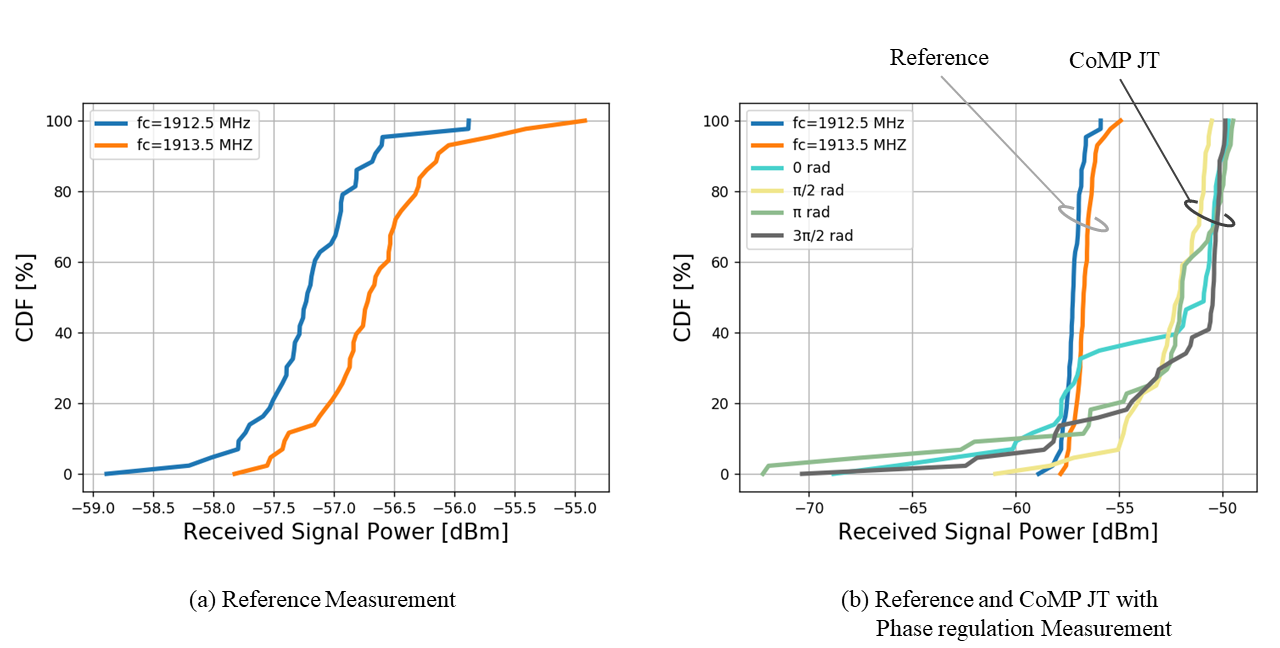
\includegraphics[width=1\textwidth]{anlagen/bilder/Abbildung1}
	\caption{Statistical analysis of the received power}
	\label{fig:Abbildung1}
\end{figure}

Ein guter Ergebnisteil erfordert Literaturzitate (vielleicht auch gar keine) und die Bekanntgabe des Ergebnisses sollte von einer Interpretation und Diskussion begleitet werden. 


\newpage

\underline{Aber \textbf{mindestens} folgende Punkte}\\
Inhalt des vierten Kapitels (im Allgemeinen):
\begin{itemize}
    \item Setzen Sie nun den Plan aus dem dritten Kapitel wenigstens prototypisch um
    \item Ziel ist es Ihre Überlegungen und Darlegungen zu beweisen
    \item Diskutieren von Problemen
    \item Zusätzlich zu der Umsetzung bedarf es (von Ihnen zu definierender) Tests, um die Funktionalität zu beweisen
    \begin{itemize}
        \item Laufzeittests, Lasttests, etc.
        \item Produzieren Sie Ergebnisse um zu zeigen, dass Ihr Ansatz funktioniert und besser/schlechter ist
        \item \glqq schlechter\grqq{} sein, bedeutet nicht, dass Ihre Arbeit schlecht ist! Am Ende zählt Ihr Ansatz und die Idee
    \end{itemize}
\end{itemize}
